% figures.tex — TikZ figures for the paper
% Included after the bibliography; figures are \input{} at appropriate places

% ============================================================
% FIGURE: Triangular decomposition and Drinfeld double
% ============================================================
\newcommand{\figTriangular}{
\begin{figure}[htbp]
\centering
\begin{tikzpicture}[node distance=1.6cm, every node/.style={font=\small}]
\node (nminus) {$u_q(\mathfrak{n}^-)$};
\node (h) [right=of nminus] {$u_q(\mathfrak{h})=\CC[G]$};
\node (nplus) [right=of h] {$u_q(\mathfrak{n}^+)=B(V)$};
\node (bminus) [below=1.1cm of nminus, xshift=1.6cm, draw, rounded corners, fill=blue!8] {$\bminus = u_q(\mathfrak{n}^-)\#\CC[G]$};
\node (bplus) [below=1.1cm of nplus, xshift=-1.6cm, draw, rounded corners, fill=red!8] {$\bplus = B(V)\#\CC[G]$};
\node (uqg) [below=2.6cm of h, draw, rounded corners, fill=green!10] {$u_q(\mathfrak{g}) \cong D(\bplus)$};
\draw[-Stealth, thick] (nminus) -- node[midway, sloped, above, font=\scriptsize]{$\#$} (bminus);
\draw[-Stealth, thick] (nplus) -- node[midway, sloped, above, font=\scriptsize]{$\#$} (bplus);
\draw[-Stealth, thick] (h) -- (uqg);
\draw[-Stealth, thick] (bminus) -- node[midway, left, font=\scriptsize]{$\otimes(\bminus)^{\mathrm{op}}$} (uqg);
\draw[-Stealth, thick] (bplus) -- node[midway, right, font=\scriptsize]{} (uqg);
\node[below=0.1cm of uqg, font=\scriptsize, text width=8cm, align=center] {Drinfeld double: $D(\bplus)=\bplus\otimes(\bminus)^{\mathrm{op}}$ with cross relations from $\langle\cdot,\cdot\rangle$};
\end{tikzpicture}
\caption{Triangular decomposition of $u_q(\mathfrak{g})$ and the Drinfeld double structure. The Cartan part $u_q(\mathfrak{h})=\CC[G]$ is shared between $\bplus$ and $\bminus$; the Nichols algebras $B(V)=u_q(\mathfrak{n}^+)$ and $u_q(\mathfrak{n}^-)$ are dual via the Hopf pairing.}
\label{fig:triangular}
\end{figure}
}

% ============================================================
% FIGURE: A_2 root system
% ============================================================
\newcommand{\figRootAtwo}{
\begin{figure}[htbp]
\centering
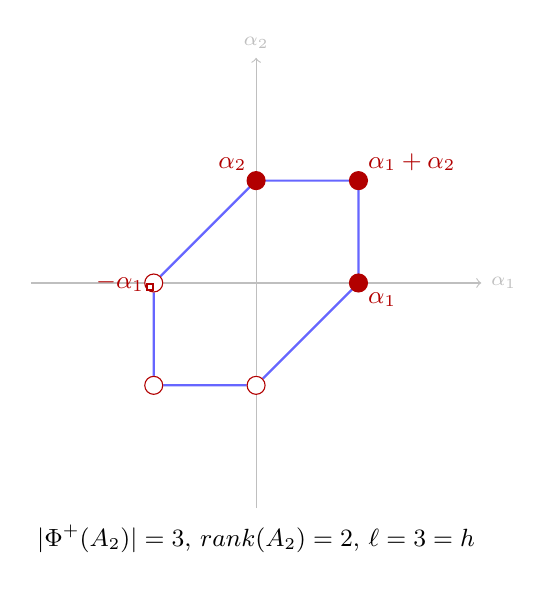
\begin{tikzpicture}[scale=1.3, every node/.style={font=\small}]
% axes
\draw[->, gray!50] (-2.2,0) -- (2.2,0) node[right, font=\scriptsize] {$\alpha_1$};
\draw[->, gray!50] (0,-2.2) -- (0,2.2) node[above, font=\scriptsize] {$\alpha_2$};
% root hexagon
\draw[blue!60, thick] (1,0) -- (1,1) -- (0,1) -- (-1,0) -- (-1,-1) -- (0,-1) -- cycle;
% positive roots (filled)
\filldraw[red!70!black] (1,0) circle (2.5pt) node[below right] {$\alpha_1$};
\filldraw[red!70!black] (1,1) circle (2.5pt) node[above right] {$\alpha_1+\alpha_2$};
\filldraw[red!70!black] (0,1) circle (2.5pt) node[above left] {$\alpha_2$};
% negative roots (open)
\filldraw[white] (-1,0) circle (2.5pt) node[below left, draw=red!70!black, thick, inner sep=1pt] {};
\filldraw[white] (-1,-1) circle (2.5pt) node[below left] {$-\alpha_1-\alpha_2$};
\filldraw[white] (0,-1) circle (2.5pt) node[below right] {$-\alpha_2$};
\draw[red!70!black] (-1,0) circle (2.5pt) node[left] {$-\alpha_1$};
\draw[red!70!black] (-1,-1) circle (2.5pt);
\draw[red!70!black] (0,-1) circle (2.5pt);
% labels
\node at (0,-2.5) {$|\Phi^+(A_2)| = 3$, $\operatorname{rank}(A_2)=2$, $\ell=3=h$};
\end{tikzpicture}
\caption{The $A_2$ root system. The three positive roots $\alpha_1, \alpha_2, \alpha_1+\alpha_2$ give $|\Phi^+|=3$; combined with $\operatorname{rank}(\mathfrak{sl}_3)=2$, the formula $\dim\HH^2=\operatorname{rank}+2|\Phi^+|=2+6=8$ is verified at $\ell=3$.}
\label{fig:rootA2}
\end{figure}
}

% ============================================================
% FIGURE: Mastnak-Witherspoon long exact sequence
% ============================================================
\newcommand{\figMWLES}{
\begin{figure}[htbp]
\centering
\begin{tikzpicture}[node distance=0.9cm, every node/.style={font=\footnotesize}]
\node (H1) {$\tilde{H}^1_b(\bplus)$};
\node (HH2) [right=of H1, draw, rounded corners, fill=green!10] {$\HH^2(u_q(\mathfrak{g}))$};
\node (HH2B) [right=of HH2] {$\HH^2(\bplus)\!\oplus\!\HH^2(\bminus)$};
\node (H2b) [right=of HH2B] {$\tilde{H}^2_b(\bplus)$};
\node (HH3) [right=of H2b] {$\HH^3(u_q(\mathfrak{g}))$};
\draw[-Stealth, thick] (H1) -- node[midway, above, font=\scriptsize]{$\delta$} (HH2);
\draw[-Stealth, thick] (HH2) -- node[midway, above, font=\scriptsize]{$\bar\iota$} (HH2B);
\draw[-Stealth, thick] (HH2B) -- node[midway, above, font=\scriptsize]{$\bar\pi$} (H2b);
\draw[-Stealth, thick] (H2b) -- node[midway, above, font=\scriptsize]{$\delta$} (HH3);
% annotation
\node[below=0.5cm of HH2, font=\scriptsize, text width=3.2cm, align=center, fill=yellow!20, rounded corners] {$\dim\im\delta=\operatorname{rank}(\mathfrak{g})$\\(Euler deriv.)};
\node[below=0.5cm of HH2B, font=\scriptsize, text width=3.2cm, align=center, fill=cyan!20, rounded corners] {$\dim\im\bar\iota=2|\Phi^+|$\\($\ell$-th power)};
\end{tikzpicture}
\caption{The Mastnak--Witherspoon long exact sequence in degree~2. The connecting homomorphism $\delta$ injects $\tilde{H}^1_b(\bplus)\cong\mathfrak{h}$ into $\HH^2(u_q(\mathfrak{g}))$, contributing the $\operatorname{rank}(\mathfrak{g})$ Cartan-type classes. The restriction map $\bar\iota$ carries the $2|\Phi^+|$ $\ell$-th power classes from $\HH^2(\bplus)\oplus\HH^2(\bminus)$.}
\label{fig:mwles}
\end{figure}
}

% ============================================================
% FIGURE: Spectral sequence E_2 page (total degree 2)
% ============================================================
\newcommand{\figSpectralSequence}{
\begin{figure}[htbp]
\centering
\begin{tikzpicture}[scale=1.1, every node/.style={font=\scriptsize}]
% grid
\foreach \q in {0,1,2} {
  \foreach \p in {0,1,2} {
    \draw[gray!40] (\p-0.5, \q-0.5) rectangle (\p+0.5, \q+0.5);
  }
}
% total degree 2 boxes highlighted
\filldraw[red!20] (-0.5, 1.5) rectangle (0.5, 2.5);
\filldraw[red!20] (0.5, 0.5) rectangle (1.5, 1.5);
\filldraw[red!20] (1.5, -0.5) rectangle (2.5, 0.5);
% labels
\node at (0,2) {$E_2^{0,2}$};
\node at (1,1) {$E_2^{1,1}$};
\node at (2,0) {$E_2^{2,0}$};
% vanish markings
\node at (0,2) [below=0.25cm] {\tiny$\HH^0(\bplus,\HH^2(\bminus))$};
\node at (1,1) [below=0.25cm] {\tiny$=0$};
\node at (2,0) [below=0.25cm] {\tiny$\HH^2(\bplus)$};
% axes
\draw[->] (-0.8,0) -- (2.8,0) node[right] {$p$};
\draw[->] (0,-0.8) -- (0,2.8) node[above] {$q$};
% total degree line
\draw[blue!60, dashed, thick] (-0.5, 2.5) -- (2.5, -0.5) node[right, font=\small] {$p+q=2$};
% d2 arrows
\draw[-Stealth, red!70!black, thick] (0.4, 2.2) -- (1.6, 1.2);
\draw[-Stealth, red!70!black, thick] (2.2, 0.4) -- (3.3, -0.5);
\node[font=\scriptsize] at (3.5, 0.8) {$d_2$};
\node[font=\scriptsize] at (1.0, 1.7) {$d_2$};
% collapse annotation
\node[font=\small, text width=6cm, align=center] at (4.5, 1.5) {Spectral sequence\\ collapses at $E_2$\\ (Theorem~\ref{thm:collapse})};
\end{tikzpicture}
\caption{The $E_2$ page of the Drinfeld double spectral sequence in total degree~$p+q=2$. The three terms $E_2^{0,2}, E_2^{1,1}, E_2^{2,0}$ are shown; $E_2^{1,1}=0$ by $\HH^1(\bminus)=0$ (Lemma~\ref{lem:hh1}), and the differentials $d_2, d_r$ ($r\geq 3$) vanish by the first-quadrant condition.}
\label{fig:ss}
\end{figure}
}

% ============================================================
% FIGURE: Decomposition of HH^2
% ============================================================
\newcommand{\figDecomposition}{
\begin{figure}[htbp]
\centering
\begin{tikzpicture}[every node/.style={font=\small, rounded corners, align=center}]
\node[draw, fill=green!15, minimum width=12cm, minimum height=1.2cm] (top) at (0,0) {$\HH^2(u_q(\mathfrak{g}),\CC)$ \quad --- \quad $\dim = \operatorname{rank}(\mathfrak{g}) + 2|\Phi^+|$};
\node[draw, fill=yellow!25, minimum width=5.5cm, minimum height=1.3cm] (left) at (-3.2,-2) {$\im(\delta) \cong \mathfrak{h}$\\ \footnotesize $\operatorname{rank}(\mathfrak{g})$ classes\\ \scriptsize Euler derivations $\Theta_i$};
\node[draw, fill=cyan!25, minimum width=5.5cm, minimum height=1.3cm] (right) at (3.2,-2) {$\im(\bar\iota)$\\ \footnotesize $2|\Phi^+|$ classes\\ \scriptsize $[E_\alpha^\ell], [F_\alpha^\ell]$};
\draw[-Stealth, thick] (-2.5,-0.6) -- (-3.2,-1.3);
\draw[-Stealth, thick] (2.5,-0.6) -- (3.2,-1.3);
\node[font=\scriptsize] at (-3.2, -0.95) {$\delta$ injective};
\node[font=\scriptsize] at (3.2, -0.95) {from $\bplus\oplus\bminus$};
% categorical
\node[draw, dashed, fill=yellow!10, minimum width=5.5cm, minimum height=0.9cm] (catL) at (-3.2,-3.6) {\scriptsize autoequivs of $D^b$\\ \tiny Cartan torus action};
\node[draw, dashed, fill=cyan!10, minimum width=5.5cm, minimum height=0.9cm] (catR) at (3.2,-3.6) {\scriptsize tensor deformations\\ \tiny truncation relations};
\draw[-Stealth, gray, thick] (-3.2,-2.7) -- (-3.2,-3.1);
\draw[-Stealth, gray, thick] (3.2,-2.7) -- (3.2,-3.1);
% geometric
\node[draw, dashed, fill=yellow!5, minimum width=5.5cm, minimum height=0.9cm] (geoL) at (-3.2,-4.8) {\scriptsize $H^2(BT,\CC)$\\ \tiny (if $\ell>h$, Ginzburg--Kumar)};
\node[draw, dashed, fill=cyan!5, minimum width=5.5cm, minimum height=0.9cm] (geoR) at (3.2,-4.8) {\scriptsize Schubert classes\\ \tiny on $G/B$};
\draw[-Stealth, gray, thick] (-3.2,-4.1) -- (-3.2,-4.3);
\draw[-Stealth, gray, thick] (3.2,-4.1) -- (3.2,-4.3);
\end{tikzpicture}
\caption{Decomposition of $\HH^2(u_q(\mathfrak{g}),\CC)$ into the $\operatorname{rank}(\mathfrak{g})$ Cartan-type classes (left) and the $2|\Phi^+|$ $\ell$-th power classes (right), with categorical and geometric interpretations. The algebraic and categorical levels are unconditional; the geometric level requires $\ell>h$.}
\label{fig:decomposition}
\end{figure}
}
